\chapter{Konzept}
\label{cha:design}

Dieses Kapitel beschreibt den theoretischen Kontext und notwendige Überlegungen, um im Kapitel \nameref{cha:implementation} die Migration problemlos umsetzen zu können. Außerdem erläutert es den nötigen Kontext, um die notwendigen Änderungen des \textit{Customerportals} nachvollziehen zu können. Namentlich handelt es sich dabei um firmeninterne Bibliotheken, die zentrale Komponenten des Systems darstellen. Ebenso zeigt es den Status Quo vor dem Projektstart und den organisatorischen Kontext.

\section{Customerportal}

Das \textit{Customerportal} ist eine 2020 entwickelte Plattform, die Firmen beim Versand von Push-Benachrichtigungen unterstützt. Benutzer:innen können Zielgruppen verwalten, Inhalte für Push-Nachrichten erstellen und bearbeiten und das Versenden dieser automatisieren. Mithilfe der \texttt{CampaignSender} Bibliothek ist es möglich, plattformunabhängig Nutzer zu benachrichtigen. Die unterstützten Plattformen belaufen sich auf iOS, Android und Google Chrome. Das Herzstück des \textit{Customerportals} ist die Oberfläche zum Orchestrieren von Push-Benachrichtigungen. Dieser Prozess ist in drei Teile unterteilt:

\begin{enumerate}
    \item \textbf{Inhalt:} Hier wählt die Nutzer:in einen Titel und den textuellen Inhalt für die zu erstellende Push-Benachrichtigung aus. Optional kann der Inhalt auch aus einer Liste von bereits erstellten Vorlagen ausgewählt werden. Inhalte können auch mit Platzhaltern versehen werden, um Nachrichten durch die Verwendung von Namen zum Beispiel zu personalisieren. Zusätzlich besteht noch die Möglichkeit, das Verhalten beim Klick auf die Benachrichtigung zu steuern. So lässt sich nicht nur die App öffnen, sondern auch gezielt auf bestimmte Unterseiten verweisen, dass zum Beispiel ein bestimmter Nachrichtenartikel geöffnet wird. Pro Plattform können beliebig viele \textit{Actions} definiert werden.
    \item \textbf{Zielgruppe:} Dieser Schritt erlaubt das Auswählen und Einschränken einer Zielgruppe. Zielgruppen können zuerst aus einer Liste von Zielgruppen ausgewählt werden. Das Erstellen neuer Einträge dieser Liste ist über den Import von CSV-Dateien möglich. Jede Person einer Zielgruppe besitzt einige Metadaten, wie zum Beispiel Sprache oder Plattform. Anhand dieser Metakriterien ist es möglich, die Zielgruppe einzuschränken. Benutzer:innen von \textit{Customerportal} ist es möglich, eigens definierte Filterkriterien anzulegen. Wünscht Resch\&Frisch etwa, dass ein neues Filterkriterium \textit{Glutenunverträglichkeit} notwendig ist, kann dieses leicht hinzugefügt werden.
    \item \textbf{Sendeverhalten:} Hier ist es abschließend noch möglich, das Absendeverhalten zu konkretisieren. Push-Benachrichtigungen können entweder sofort, zu einem fixen Zeitpunkt in der Zukunft oder in regelmäßigen Intervallen auf täglicher oder wöchentlicher Basis versendet werden.
\end{enumerate}

Das \textit{Customerportal} kann entweder selbst betrieben oder als von \textit{Cloudflight} betrieben SaaS-Lösung verwendet werden. \textit{Cloudflight} bietet zur Basis-Applikation noch Zusatzmodule, die den Funktionsumfang erweitern. Zu den Kunden des \textit{Customerportals} zählen unter anderem Resch\&Frisch, Linz AG und Abfall OÖ. 

Original unter \textit{mogree} entwickelt, ging das \textit{Customerportal} 2022 mit dem Verkauf von \textit{mogree} an \textit{Cloudflight} automatisch auch in deren Besitz über. Seit der originalen Entwicklungsarbeit 2020 wurden kaum Instandhaltungsmaßnahmen daran vorgenommen, was sich nunmehr drei Jahre später zeigt. Schwerwiegende Sicherheitslücken wie CVE-2021-44228 (\textit{Log4Shell}) wurden seither entdeckt und stellen ein fortbestehendes Sicherheitsrisiko dar~\parencite{cvelog4shell}. Mit 2023 gilt es nun, eine aktualisierte Version des \textit{Customerportals} zu erstellen.

\section{Projektkontext}

Der Startschuss für dieses Projekt wurde mit der dritten Woche des Berufspraktikums angesetzt, nachdem die bisherige Aufgabe des \textit{mathe2go} Projektes abgeschlossen werden konnten. Die Abnahme der geleisteten Arbeit erfolgt durch den Vorgesetzten Andreas Schweiger, der auch schon 2020 technische Führungskraft war.

Große Teile der Arbeit wurden auf selbstständiger Basis erledigt. Bei Pull-Requests und technischen Diskussionen erfolgte die Zusammenarbeit mit dem Kollegen Johannes Krenn, der momentan nebenberuflich zum Master-Studium an der FH Hagenberg noch bei Cloudflight tätig ist.

\section{Projektarchitektur}

Das zentrale System des Customerportals ist das Backend in Form einer Spring Boot Applikation. Das Backend stellt eine REST-Api zur Verfügung. Der Zugriff darauf ist entweder durch die REST-Api direkt oder mit dem Angular Frontend als Benutzeroberfläche möglich. Zusätzlich sind viele Funktionen und Mechanismen auf eigens entwickelte Bibliotheken ausgelagert.~\autoref{fig:c4-cp} zeigt das C4-Modell der Komponenten des \textit{Customerportals}.

\begin{figure}[h]
    \caption{C4-Modell des \textit{Customerportals}}
    \centering
    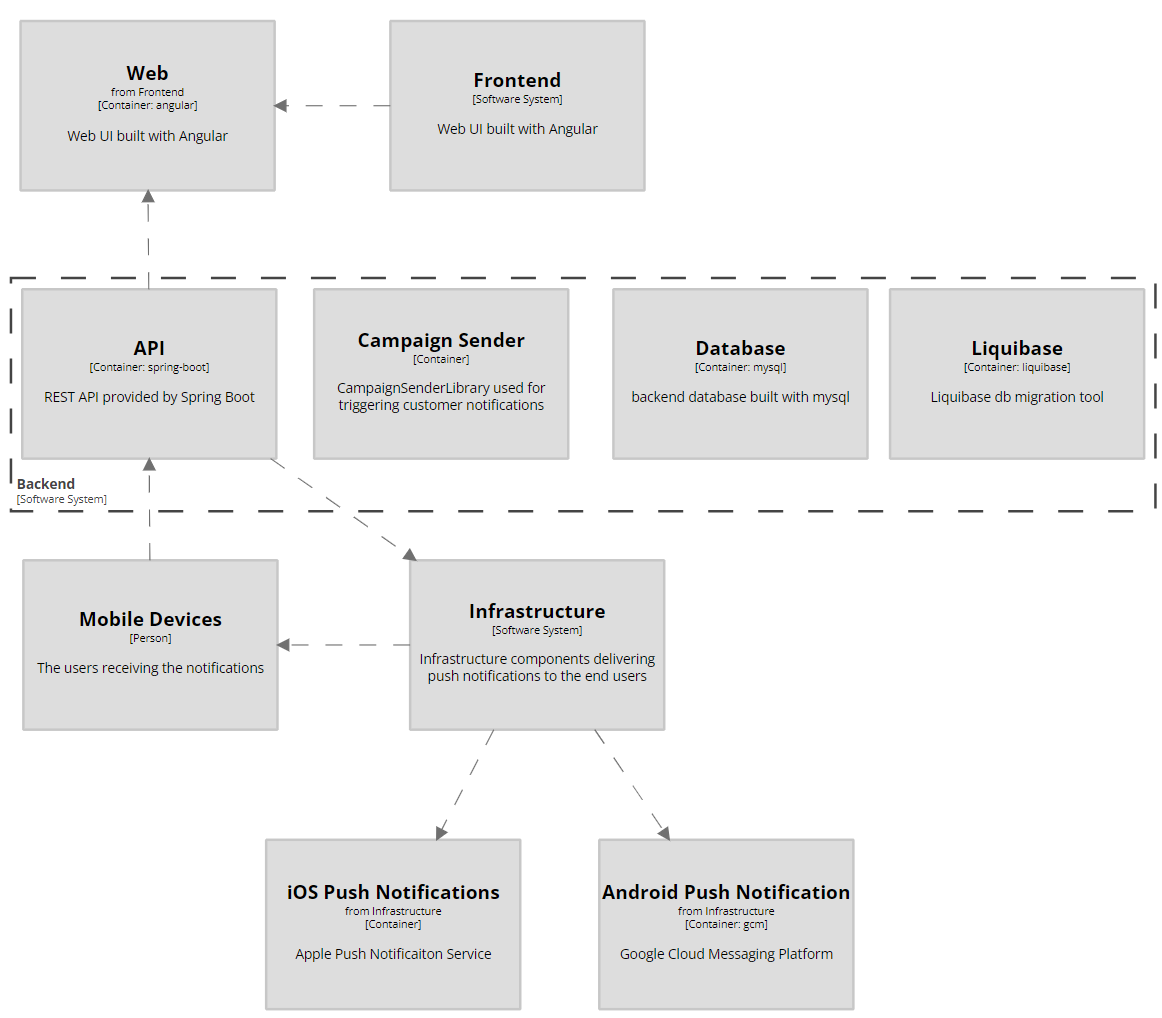
\includegraphics[width=\textwidth]{C4.Architecture.System}
    \label{fig:c4-cp}
\end{figure}

\subsection{Backend}

Das Backend umfasst mehrere wichtige Komponenten mit einer Spring Boot-Applikation im Zentrum. Dieses Backend stellt eine REST-Api zur Verfügung und nutzt OAuth2.0 zum Authentifizieren von Nutzern und zum Autorisieren von Zugriffen auf die Schnittstelle. Clients authentifizieren sich durch die Präsenz eines \texttt{Authorization}-Headers in der Http-Anfrage. Diesen Header erhält ein Client nach dem erfolgreichen Anmelden.

Eine MySql Instanz dient zum Persistieren der Daten. Liquibase wendet Migrationen auf die Datenbank an und befüllt diese mit Test-Daten, wenn es im Kontext einer Test-Umgebung ausgeführt wird. Sowohl die lokale Mysql-, als auch die Liquibase-Instanz laufen in Docker-Containern, die von einem Docker-Compose-Script orchestriert werden.

Benutzer und deren personenbezogene Daten werden verschlüsselt in der Datenbank gespeichert. Dadurch ist keine Nachverfolgung von bestimmten Nutzern möglich, sollte etwa ein Datenleck auftreten. Jedoch ist weiterhin die Anwendung von Filtern, wie zum Beispiel die Einschränkung der Altersgruppe möglich. 

Lokal wird das Backend typischerweise mit Intellij IDEA ausgeführt. Dasselbe gilt auch für die JUnit-Tests. Alternative kann das Customerportal jedoch auch containerisiert ausgeführt werden. Dadurch kann die Infrastruktur des Produktionssystem lokal simuliert werden.

Wichtige Teile des Backends sind auf private Bibliotheken, die mit Artifactory verwaltet werden, ausgelagert. Allen voran \texttt{mogree-codegen} zum Erzeugen der REST-Api. Die Bibliothek erzeugt auf Basis einer Spezifikation in einer Swagger-konformen yaml-Datei die Klassen der Schnittstelle. Dadurch muss nur die Logik eines Endpunktes in einem \texttt{Service} definiert werden. Meta-Informationen, wie zum Beispiel Swagger-Annotationen generiert die Bibliothek auf Basis der Spezifikationsdatei. Zum Erzeugen der REST-Api Quelldateien verwendet \texttt{mogree-codegen} \texttt{mustache}-Dateien als Schablone: Statische Textstücke sind direkt in der Datei enthalten. Variable Textfragmente, die sich je nach Endpunkt unterscheiden, haben im Text einen Platzalter (doppelte geschwungene Klammer - wie Angular). Bei der Übersetzung erzeugt die Bibliothek ein Modell, anhand welchem die Platzhalter durch Werte der Variablen ersetzt werden.

Ist zum Beispiel in einer Datei \texttt{swagger.yml} ein Endpunkt \texttt{/account/login} spezifiziert, wird die Schnittstelle \texttt{AccountDelegate} und die Klasse \texttt{AccountController} erzeugt. Beide Typen enthalten eine Funktion \texttt{login}. Der/Die Entwickler:in muss nun eine Klasse \texttt{AccountService} definieren, die \texttt{AccountDelegate} implementiert. Zusätzlich noch wird die Implementierung durch \texttt{@Component} zu einer injezierbaren Komponente in Spring und mit \texttt{@Primary} als Hauptimplementierung der Schnittstelle markiert. Die Klasse \texttt{AccountController} erhält nun die Implementierung der Delegateklasse aufgrund der Dependency-Injection-Mechanismen von Spring. Fehlercodes, wie zum Beispiel 401 (Unauthorized) werden durch Ausnahmezustände repräsentiert. Das Diagramm~\autoref{fig:codegen-diagram} zeigt diesen Prozess. \texttt{Mogree-codegen} erzeugt die folgenden vier Pakete:

\begin{itemize}
    \item \texttt{api}: Hier liegen die Controller der REST-Api. Jeder Controller implementiert eine Schnittstelle, die den Suffix -Api trägt und die Swagger-Annotationen enthält. Außerdem befindet sich hier der Delegate des Controllers .
    \item \texttt{config}: Hier liegt die Konfiguration der Swagger-UI.
    \item \texttt{model}: Dieses Paket enthält die DTOs, die an den Client zurückgesendet werden.
    \item \texttt{param}: Hier liegen die Param-Objekte, die an die Delegate-Implementierungen übergeben werden.
\end{itemize}

\texttt{Mogree-codegen} ist ein \textit{fork} der Bibliothek~\textcite{githubswaggercodegen}, da sie nicht alle Anforderungen erfüllte. Wie in~\autoref{lst:account_rest} zu sehen ist, erzeugt die \texttt{login}-Methode auf Basis der Parameter ein Objekt des Typs \texttt{ParamLogin} und übergibt es an die Implementierung des Delegates. Diese Param-Objekte werden in \texttt{swagger-codegen} nicht erzeugt, wodurch dieser \textit{fork} nötig war. Auf die Nachteile des selbst entwickelten Ansatzes geht dieser Bericht im weiteren Verlauf noch ein.

\begin{JavaCode}[numbers=none, caption={Der generierte \texttt{AccountController}}, label=lst:account_rest]
@RestController
public class AccountController implements AccountApi {
    ...
    public ResponseEntity<DetailResponse<UserAuthModel>> login(
            @Parameter(description = "Email of user", required = true)
            @RequestHeader(value = "mogree-Mail", required = true)
            String mogreeMail,
            @Parameter(description = "Password of user", required = true)
            @RequestHeader(value = "mogree-Password", required = true)
            String mogreePassword
    ) {
        ParamLogin paramLogin = new ParamLogin(mogreeMail, mogreePassword);
        return new Executer(validators).validate().usecase(() -> delegate.login(paramLogin)).run();
    }
}
\end{JavaCode}

Die Konfiguration des Zielverzeichnisses, des Vorlagenverzeichnisses und der Spezifikationsdatei erfolgt durch Gradle in der \textit{Task} \texttt{codegenConfig}. Diese \textit{Task} erfolgt in der Ausführungsphase von Gradle und wird dadurch bei jeder Kompilation ausgeführt~\parencite{gradlelifecycle}.

\begin{figure}[h]
    \caption{Ablauf der Codegenerierung anhand des Beispiels des AccountControllers.}
    \centering
    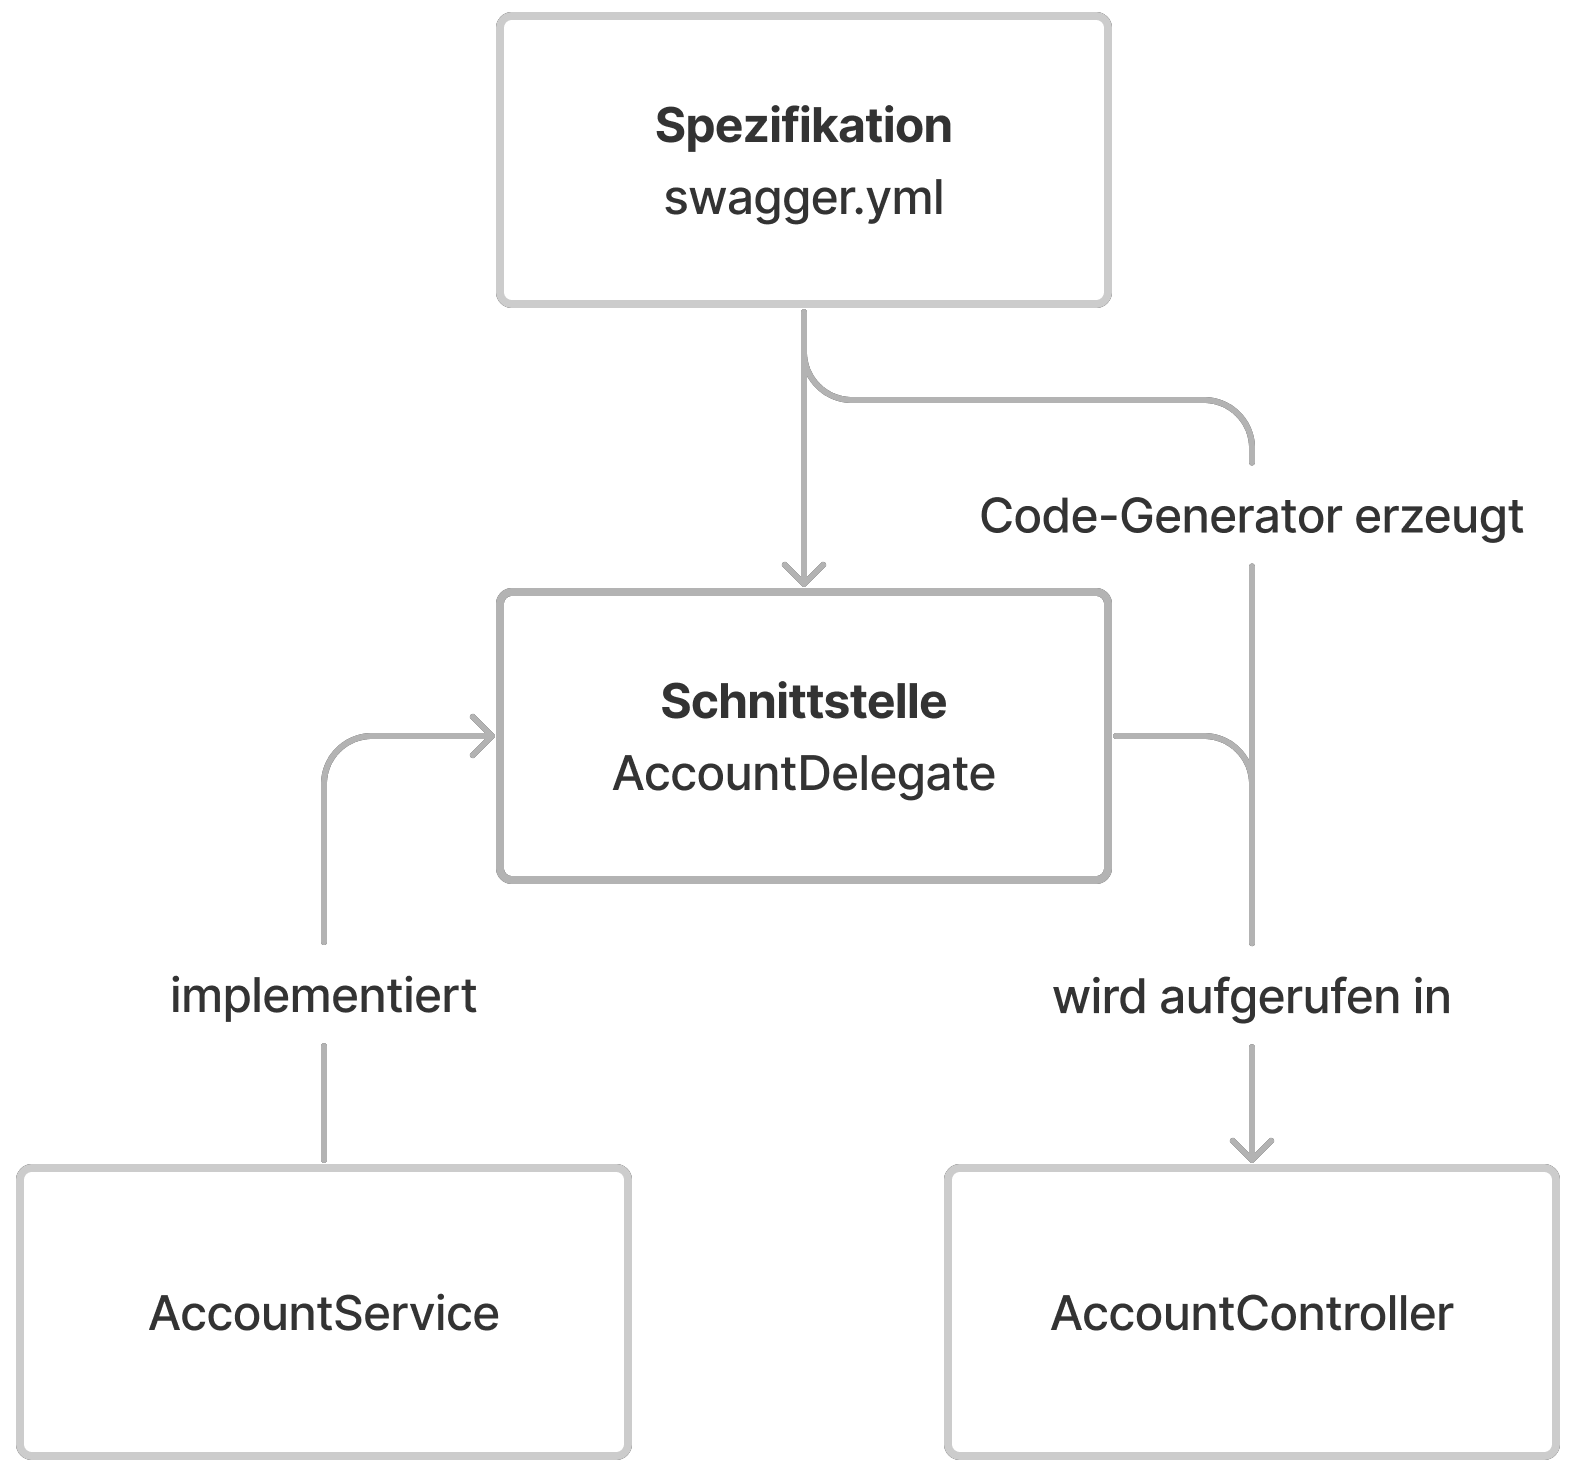
\includegraphics[scale=0.4]{Code.Generator}
    \label{fig:codegen-diagram}
\end{figure}

Neben \texttt{mogree-codegen} kommen noch weitere Bibliotheken zum Einsatz. Die Bibliothek \texttt{mogree-spring} bietet in vielen Teilbereichen von Spring Erweiterungen und Verbesserungen. So sind die \texttt{Validators}, die in~\autoref{lst:account_rest} zu sehen sind, in der Bibliothek enthalten. Ebenso werden auch viele Klassen und Schnittstellen, die bei der Verarbeitung von Client-Anfragen benötigt werden über \texttt{mogree-spring} bereitgestellt.

Die Bibliothek \texttt{library-jwt} enthält die Authentifizierungs- und Autorisierungslogik. Wie bereits erwähnt wird hierfür OAuth2.0 mit JWT verwendet. Außerdem übernimmt die Bibliothek die Einordnung der Autorisierungs-Filterregeln in der Spring \texttt{HttpSecurity}-Filterkette. Sollte im Autorisierungsprozess ein Ausnahmezustand auftreten, so übernimmt \texttt{library-jwt} die Behandlung davon.

Das Backend verwendet die Bibliothek \texttt{springfox} zum Bereitstellen der Swagger-UI. Swagger-UI dient zum Visualisieren der REST-Api. Die Benutzeroberfläche dafür ist unter dem Pfad \texttt{/api/v1/swagger-ui.html} im Browser verfügbar. Damit können Anfragen an den Server getätigt werden und die Antwort betrachtet werden.

\subsection{Frontend}
\label{sec:design-frontend}

Das Frontend ist eine Weboberfläche, die mit dem Framework Angular implementiert ist. Sie greift auf das Backend durch die Api zu. Die Komponenten der Benutzeroberfläche bauen auf Angular-Material-Komponenten auf, wobei teilweise Style-Änderungen vorgenommen wurden.~\autoref{fig:cp-web-home} zeigt die Startseite des Frontends.

\begin{figure}[h]
    \caption{Die Startseite des Customerportal-Frontends, die der/die Benutzer:in nach dem Login zu sehen bekommen.}
    \centering
    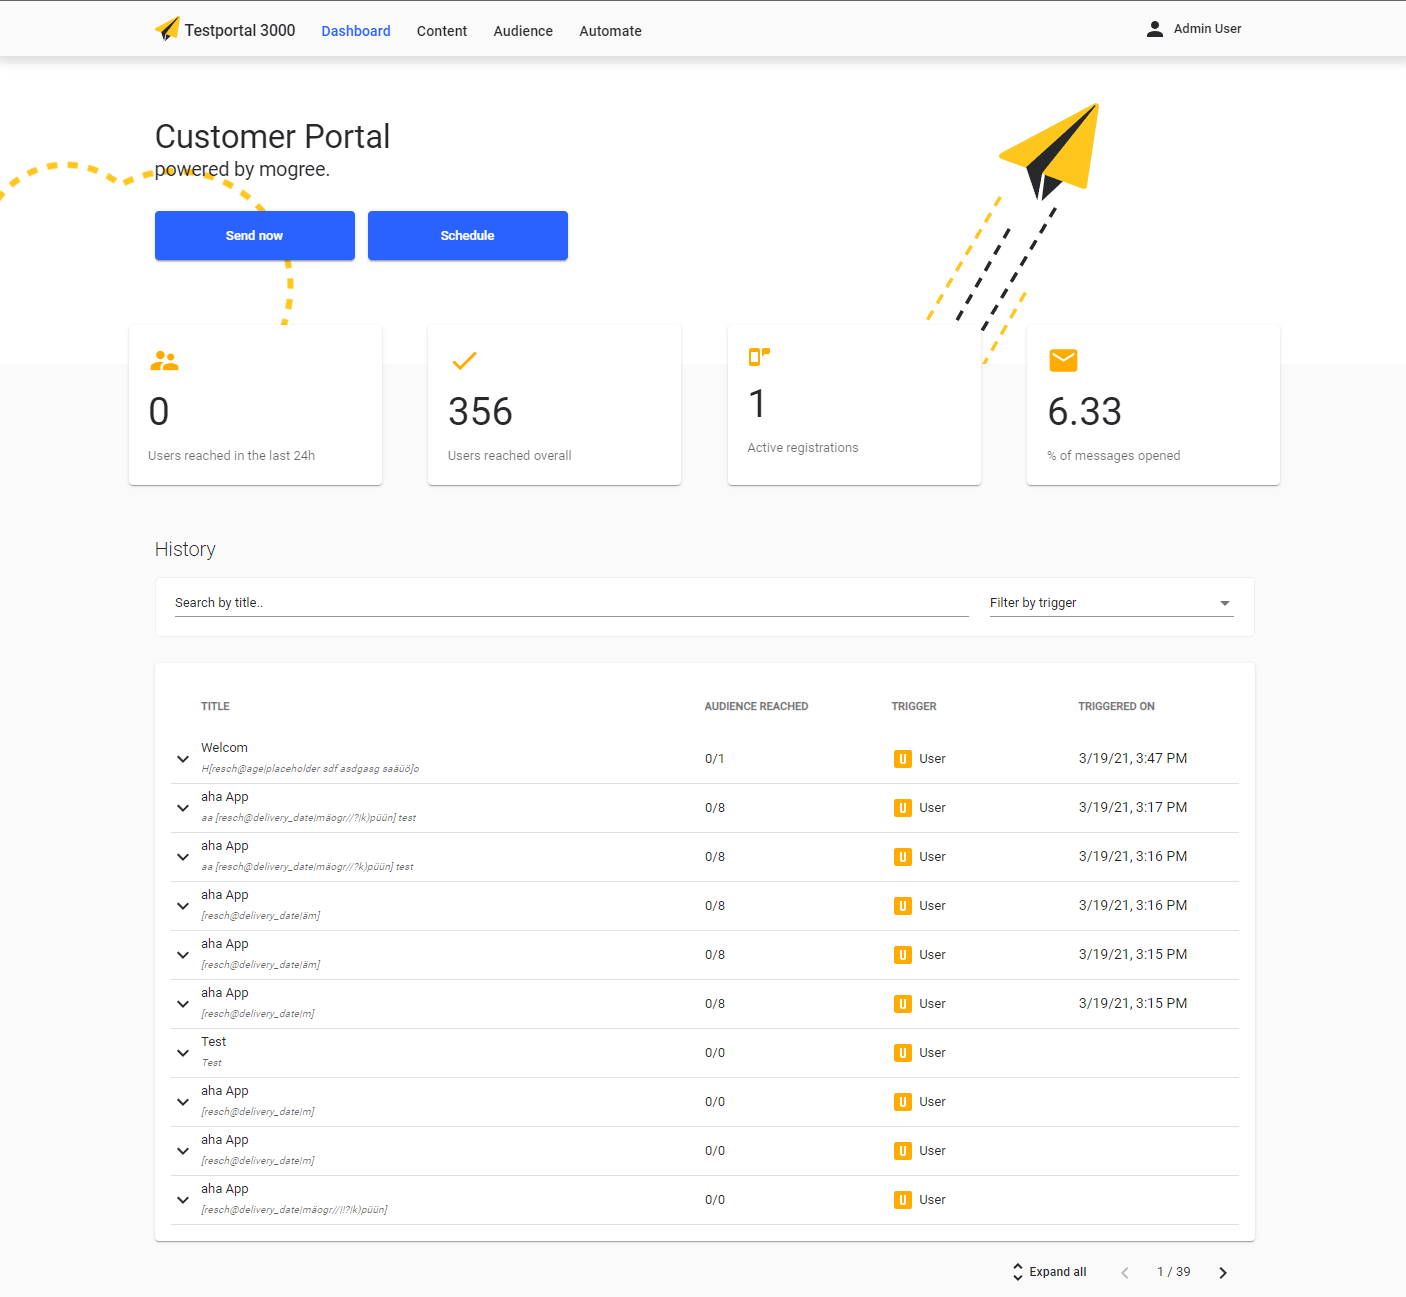
\includegraphics[scale=0.38]{CP.Web.Home}
    \label{fig:cp-web-home}
\end{figure}

Programmatisch ist das Frontend in einem desolaten Zustand. Viel Code ist hier schlecht geschrieben und sollte überarbeitet werden. Vor allem sind Komponenten oft viel zu groß. Teilweise überschreiten Viewmodel-Klassen die 1000-Zeilen Hürde. In solchen Fällen wäre eine Aufspaltung in mehrere kleinere Komponenten ratsam. Dadurch erhöht sich die Wiederverwendbarkeit und Lesbarkeit des Systems.

Der Codequalität ist auch auf der Mikro-Ebene schlecht. Funktionslogik hat oft eine höhere Komplexität als nötwendig oder sinnvoll. Teilweise sind Funktionen über 300 Zeilen lang und haben eine dreistellige zyklomatische Komplexität. 

\subsection{Infrastruktur}

Alle Bibliotheken und Systemkomponenten verwenden eine im Intranet stationierte Gitlab-Instanz zur Versionsverwaltung. Das Branching-Modell entspricht dem Gitflow-Modell von Atlassian~\parencite{gitflow}.

Als CI/CD-Werkzeug wird eine ebenso selbst verwaltete Jenkins-Instanz betrieben. Ein Push auf den \texttt{develop} oder \texttt{master}-Branch löst eine Routine in Jenkins aus, welche die Tests ausführt, ein Kompilat erzeugt und dieses auf den Test- oder Produktivsystem spielt. Die Implementierung der Routinen befindet sich in der Datei \texttt{Jenkinsfile} im Wurzelverzeichnis des Git-Repository. Diese Datei bekommt noch besondere Relevanz hinsichtlich der Verwaltung von sensiblen Daten im Laufe der Arbeit.

\section{Behandlung von sensiblen Daten}
\label{sec:design_sensitive_data}

Bei der Behandlung von sensiblen Daten geht es um die Entfernung von Passwörtern, Benutzernamen, etc. aus dem Code und die Ersetzung durch Variablen. Bisher waren diese hart kodiert in den Konfigurationsdateien des Backends vorhanden. Es gilt diesen Prozess sicherer zu gestalten.

\subsection{Ausgangslage}

Bisher wurden sensible Daten direkt in den Konfigurationsdateien (mit yaml Syntax) von Spring Boot gelagert. Darunter fallen Datenbankzugangsdaten, Emailpasswörter und JWT-Schlüssel. Das kann zu gefährlichen Sicherheitslücken führen, sollte in einen Teil der Entwicklungskette von Dritten eingedrungen werden. Konkret könnten Angreifer die Daten in Gitlab, im Quelltext, in Jenkins oder in den Produktiv- und Entwicklungssystem erlangen, um in weiterer Folge Schaden mit den Zugangsdaten anzurichten. Ein weiterer Nachteil ist die Umständlichkeit beim Ändern der Daten. Ändert sich zum Beispiel ein Datenbankpasswort, muss der Quelltext der Konfiguration bearbeitet und der ganze erneut Build-Prozess durchlaufen werden, um das Passwort zu ändern.

\subsection{Vorgangsweise}

Diesen Prozess gilt es nu zu verbessern. Ziel ist es, dass im Quelltext anstatt sensibler Daten nun Platzhalter vorhanden sind. Außerdem sollen die Daten an einem zentralen Ort bearbeitet, angelegt und gelöscht werden können. Der Grundgedanke dieser Aufgabe ist, sensible Daten als Umgebungsvariablen in den Docker Container zu injizieren. Ebenso sollen die Daten auch an einer zentralen Stelle gut wartbar sein, weshalb die direkte Lagerung am Server ausgeschlossen werden kann. Die Herausforderung dabei ist die Vielzahl an Umgebungen, durch die die Daten transportiert werden müssen.

\subsubsection{Spring Konfiguration}

Die Konfigurationsdateien von Spring sollen komplett von allen sensiblen Daten befreit werden. In Zukunft sollen sich hier keine Werte oder nur noch Platzhaltervariablen befinden. Dafür gibt es mehrere Ansätze:

\begin{itemize}
    \item \textbf{Zeichenketteninterpolation:} Die Konfigurationsdateien von Spring erlauben Zeichenketteninterpolation mit der Groovy-Syntax \texttt{\$\{\}}. Zwischen den geschwungenen Klammern kann der Name einer Umgebungsvariablen platziert werden, wodurch der Wert der Variable interpoliert wird. So interpoliert der Ausdruck \texttt{\$\{JAVA\_HOME\}} den Wert der Umgebungsvariable \texttt{JAVA\_HOME}. Durch die Syntax \texttt{\$\{<variable-name>:<default-value>\}} kann zusätzlich ein Standardwert angegeben werden, sollte die Variable keinen Wert aufweisen~\parencite{springpropertyplaceholder}.
    \item \textbf{Direkte Verwendung von Umgebungsvariablen:} Alternative ist es auch möglich, einzelne Variablen der Spring Konfiguration völlig aus den yaml-Dateien auszulagern~\parencite{springexternalizedconfig}. Spring setzt genau fest, in welcher Reihenfolge wo nach Variablen gesucht wird, sollte die Variable nicht am nächsthöheren Ort vorhanden sein. Bei Umgebungsvariablen wird hierbei eine genaue Syntax vorausgesetzt~\parencite{springbindingenvvariables}. Punkte sind durch Unterstriche zu ersetzen, Bindestriche müssen entfernt werden und Kleinbuchstabe müssen durch Großbuchstaben ersetzt werden. So ist der Wert des Schlüssels \texttt{spring.mail.sender} in der Umgebungsvariable \texttt{SPRING\_MAIL\_SENDER} zu finden.
\end{itemize}

Die Entscheidung fiel hierbei auf die direkte Verwendung von Umgebungsvariablen. Der Grund und die Umsetzung davon wird im Kapitel~\nameref{cha:implementation} näher erläutert.

\subsubsection{Jenkins Konfiguration}

Die tatsächliche Logik der Jenkins-Pipeline liegt in der Datei \texttt{Jenkinsfile} im Wurzelverzeichnis des Customerpotal-Repository. Bevor die Pipeline aber um die nötige Logik erweitert werden kann, müssen die Umgebungsvariablen an einem leicht zugänglichen und verwaltbaren Ort abgelegt werden. Dafür bietet sich die Weboberfläche von Jenkins sehr gut an.

In der Weboberfläche existieren zwei Möglichkeiten, wie die Zugangsdaten gelagert werden können. Die erste Möglichkeit -- die nicht gewählt wurde -- ist die Verwendung des \textit{Credentials}-Speicher in dem Werttupel in einem gewissen Schema gespeichert werden können.

Alternativ dazu besteht die Möglichkeit der Anlage von \textit{Config}-Dateien in der Weboberfläche. Diese können Text in beliebiger Form enthalten. Da es sich beim Produktiv- und Testsystem um Linux-Server handelt, würde sich das Format \texttt{<key>=<value>} in jeder Zeile gut anbieten, da es der Syntax des Befehls \texttt{export} entspricht~\parencite{archwikienvfiles}.

Die Entscheidung hierbei fällt auf den Ansatz mit \textit{Config}-Dateien. Sie bieten mehr Flexibilität und die Benutzeroberfläche ist besser zur Verwaltung der Daten geeignet.

\subsubsection{Jenkins Pipeline}

Die Jenkins Pipeline hat die Aufgabe, die Dateien, die die Umgebungsvariablen enthalten, von Jenkins-System an die Test- und Produktivsysteme zu übertragen. Ebenso muss auch die dynamische Konfiguration für einzelne Kundensysteme möglich sein. So soll zum Beispiel ein Produktivsystem für Resch\&Frisch keine sensiblen Daten von AbfallOÖ enthalten. Für diesen Zweck kommen \textit{Parametrized Builds} zum Einsatz~\parencite{jenkinsparametrizedbuilds}. Auf Basis der Auswahl aus einer Liste von Werten werden dann die richtigen Dateien geladen.

Weiß man nun die Namen der richtigen Dateien, müssen diese vom Build-System auf die Test- und Produktivsysteme übertragen werden. Dafür wird das Kommandozeilen-Werkzeug \texttt{ansible} verwendet, da es bereits zum Übertragen der \texttt{jar}-Datei verwendet wird. \texttt{Ansible} ist ein Werkzeug von Red Hat zur Verwaltung von Infrastruktur durch Code~\parencite{redhatansible}.

\subsubsection{Docker Konfiguration}

Zu diesem Zeitpunkt sind nun die Umgebungsvariablen in den \texttt{env}-Dateien auf den Test- und Produktivsystemen, aber noch nicht im Docker Container des Backends. Daher muss abschließend noch die \texttt{Dockerfile} bearbeitet werden, dass die Umgebungsvariablen aus den Dateien in den Container exportiert werden. Die Logik hierfür muss sich entweder im Befehl \texttt{ENTRYPOINT} oder \texttt{RUN} befinden, da diese Befehle im Container und nicht während dem Build-Prozess ausgeführt werden. Zum Setzen der Umgebungsvariable bietet Linux den Befehl \texttt{export <key>=<value>}.

\section{Aktualisierung Spring Boot}

Der zweite Teil der Hauptaufgabe befasst sich mit der Migration von Spring Boot 2 auf 3. Außerdem müssen öffentliche Bibliotheken auf den neuesten Stand gebracht werden und private Bibliotheken mit Spring Boot 3 kompatibel gemacht werden.

\subsection{Ausgangslage}

Das Backend des Customerportals wurde 2020 mit der neuesten Spring Boot Version entwickelt. Das war damals die Version \texttt{2.3.2.RELEASE}. Seither wurden sowohl bei Spring als auch bei Bibliotheken keine Aktualisierung vorgenommen. Kotlin selbst war noch bei Version 1.4.31, während die aktuelle Version schon bei 1.8.21 ist. Mit immer wieder bekanntwerdenden Sicherheitslücken und der Veröffentlichung von Spring Boot 3 soll das Customerportal nun aktualisiert werden.

\subsection{Vorgangsweise}

Die Migration wird auf Basis von~\parencite{baeldungspring3migration} und~\parencite{githubspringmigration} vorgenommen. In einem ersten Schritt muss Spring Boot auf die Version 2.7.11 und Spring Security auf Version 5.8 aktualisiert werden. Beides sind die neuesten Versionen vor dem Sprung von Version 2 auf Version 3.

Nachdem Spring Boot und Spring Security auf ihre Zwischenversionen aktualisiert worden sind, müssen nun die Abhängigkeiten auf den neuesten Stand gebracht werden. Hier ist besondere Vorsicht geboten, da bei der Menge der Abhängigkeiten, die das Backend aufweist, ein komplexer Abhängigkeitsgraph die Folge ist. Ist nun zum Beispiel eine Komponente mit einer anderen Komponente nicht mehr kompatibel, kann die Fehlerquelle oft nur schwer eruiert werden, da Gradle Fehlermeldungen oft irreführend und wenig hilfreich sind. Daher müssen die Versionen der Abhängigkeiten sehr granular und mit vielen Tests aktualisiert werden. Seit der originalen Entwicklung sind nunmehr drei Jahre vergangen, weshalb die neuesten Versionen der Bibliotheken mittlerweile oft \textit{Breaking Changes} aufweisen, weshalb bei jeder Bibliothek das Änderungsprotokoll durchzulesen ist.

Nachdem die öffentlichen Bibliotheken nun auf dem aktuellen Stand sind, können nun die privaten Bibliotheken aktualisiert werden. Die Bibliotheken \texttt{mogree-spring} und \texttt{library-jwt} bauen auf Spring Boot auf, weswegen hierfür auch die Migration auf Spring Boot 3 durchzuführen ist. Bei \texttt{mogree-codegen} muss an einigen Stellen der Code angepasst werden.

Spring Boot 3 fordert von Gradle die Mindestversion 7.5~\parencite{springbootgradleminversion}, weswegen Gradle auf Version 8.1 aktualisiert werden sollte. Außerdem verlangt Spring Boot 3 bei Kotlin die Mindestversion 1.7 und bei Java Version 17. In Kombination mit dem Kotlin Annotationsprozessor (kapt) kommen hierbei im Kapitel~\nameref{cha:implementation} noch Probleme auf.

Abschließend muss die Aktualisierung auf Spring Boot 3 beim Customerportal selbst durchgeführt werden. Hier muss Hibernate von Version 5 auf Version 6 und Spring Security von Version 5.8 auf Version 6 aktualisiert werden. Das erfolgt auf Basis von~\parencite{hibernate6migration} und~\parencite{springsecurity6migration}.

Springfox wurde bisher zum Generieren der Api-Dokumentation verwendet, bietet aber keine Unterstützung für Spring Boot 3 an. Daher muss Springfox durch eine andere Bibliothek ersetzt werden. Die etablierte Standardlösung für Spring Boot ist die Bibliothek Springdoc und soll auch beim Customerportal zum Einsatz kommen. Infolgedessen müssen die \texttt{mustache}-Vorlagen von der Swagger2.0-Annotation auf die OpenAPI-Annotation umgeschrieben werden.

\section{Aktualisierung Angular}

Wie in~\nameref{sec:design-frontend} beschrieben wurde, ist die Codequalität der Angular-Applikation unzufriedenstellend. Komponenten gehören überarbeitet und aufgeteilt. Aufgrund des mangelnden wirtschaftlichen Nutzens des Frontends werden jedoch nur kleine kosmetische Änderungen vorgenommen, sodass der bisherige Zustand des Frontends erhalten bleibt. Regressionen, die durch die Aktualisierung auf Angular 14 anfallen, sind jedoch zu beheben. Eine Aktualisierung auf Angular 15 oder 16 ist wirtschaftlich ebenso wenig sinnvoll, da große Änderungen am Style vorzunehmen. Daher bleibt es bei der Aktualisierung von Angular 10 auf 14.

Mit einem konkreten Plan bezüglich der Aktualisierung des Customerportal-Backends kann nun die Umsetzung davon begonnen werden. Das nächste Kapitel zeigt die Schritte, die zur Implementierung nötig sind.